\chapter[TKM: a temporal knowledge model]{TKM: a temporal knowledge model to represent actions, their contexts and their impacts}
\chapterPage{
The evolving complexity of adaptive systems impairs our ability to deliver anomaly-free solutions. 
Fixing these systems require a deep understanding on the reasons behind decisions which led to faulty or suboptimal system states. 
Developers thus need diagnosis support that trace system states to the previous circumstances –targeted requirements, input context– that had resulted in these decisions. 
However, the lack of efficient temporal representation limits the tracing ability of current approaches. 
To tackle this problem, we first propose a knowledge formalism to define the concept of a decision. 
Second, we describe a novel temporal data model to represent, store and query decisions as well as their relationship with the knowledge (context, require- ments, and actions). 
We validate our approach through a use case based on the smart grid at Luxembourg. We also demonstrate its scalability both in terms of execution time and consumed memory.
 }
 
 \section{Introduction}
 
should define: decision, action, context, knowledge
 
 \section{Knowledge formalization}
 
  As discussed previously, I consider \gls{knowledge} to be the association of \gls{context} information, \glspl{requirement}, and \gls{action} information, all in one global and unified model.
 While \gls{context} information captures the state of the system environment and its surroundings, the system \glspl{requirement} define the constraints that the system should satisfy along the way. 
 The \glspl{action}, on the other hand, are means to reach the goals of the system.
  
 In this section, I provide a formalization of the \gls{knowledge} used by adaptation processes based on a temporal graph. 
Indeed, due to the complexity and interconnectivity of system entities, graph data representation seems to be an appropriate way to represent the \gls{knowledge}. 
Augmented with a temporal dimension, temporal graphs are then able to symbolize the evolution of system entities and states over time. 
We benefit from the well-defined graph manipulation operations, namely temporal graph pattern matching and temporal graph relations to represent the traceability links between the \glspl{decision} made and their \glspl{circumstance}.

Before describing this formalism, I describe the semantic used for the temporal axis.
Then, I exemplify the knowledge formalism using the Luxembourg smart grid use case.

\subsection{Formalization of the temporal axis}
\label{sec:tkm:timeDef}

\begin{figure}
   \centering
	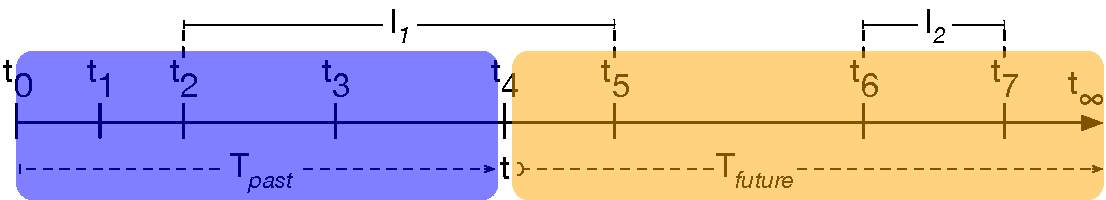
\includegraphics[width=\textwidth]{img/chapt-tkm/formalismeTime}
	\caption{Time definition used for the knowledge formalism}
	\label{fig:tkm:formalismeTime}
\end{figure}

The formalism describe below has been made with two goals in mind.
First, the definition of the time space should allow the distinction between past and future. 
Doing this distinction enable the differentiation between measured data and estimated (or predicted data).
Second, it should permit the definition of the life cycle of an element of the \gls{knowledge}, which can be seen as a succession of states with a validity period that should not overlap each other.

Time space $T$ is considered as an ordered discrete set of time points non-uniformly distributed. 
As depicted in Figure~\ref{fig:tkm:formalismeTime}, this set can be divided into 3 different subsets $T = T_{past} \cup \{t\} \cup T_{future}$, where:  
\begin{itemize}
	\vspace{-0.5em}
	\setlength\itemsep{-0.3em}
	\item $T_{past}$ is the sub-domain \{$t_{0}$;$t_{1}$;\ldots;$t_{current-1}$\}  representing graph data history starting from $t_0$, the oldest point, until current time, t, excluded.
	\item \{t\} is a singleton representing the current time 
point
	\item $T_{future}$ is sub-domain \{$t_{current+1};\ldots;t_{\infty}$\} representing future time points 
\end{itemize}
The three domains depend completely on the current time \{t\} as these subsets slide as time passes. 
At any point in time, these domains never overlap: $T_{past} \cap \{t\} = \emptyset$, $T_{future} \cap \{t\} =  \emptyset$, and $T_{past} \cap T_{future} = \emptyset$.
The definition of these three subsets reachs the first goal.

In addition, there is a right-opened time interval $I \in T \times T$ as $[t_s, t_e)$ where $t_e - t_s > 0$.
In English words, it means that the interval cannot represent a single time point and should follow the time order. 
For any $i \in I$, $start(i)$ denotes its lower bound and $end(i)$ its upper bound.
As detailed in Section~\ref{sec:tkm:formalism}, these intervals are used to define the validity period for each node of the graph. 

Figure~\ref{fig:tkm:formalismeTime} displays an example of a time space $T_1 = \{t_0, t_1, t_2, t_3, t_4, t_5, t_6, t_7\}$.
Here, the current time is $t = t_4$.
According to the definition of the past subset ($T_{past}$) and the future one ($T_{future}$), there is: $T_{past1} =  \{t_0, t_1, t_2, t_3\}$ and $T_{future1} = \{t_5, t_6, t_7\}$.
Two intervals have been defined on $T_1$, namely $I_1$ and $I_2$.
The first one starts at $t_2$ and ends at $t_5$ and the last one is defined from $t_6$ to $t_7$.
As shown with $I_1$, an interval could be defined on different subsets, here it is on all of them ($T_{past}$, $t$, and $T_{future}$).

\subsection{Formalism}
\label{sec:tkm:formalism}
 
 \paragraph{Graph definition}
First, let $K$ be an adaptive process over a system \gls{knowledge} represented by a graph such as $K = (N, E)$, comprising a set of nodes $N$ and a set of edges $E$.
Nodes represent any element of the knowledge (context, actions, \etc) and edges represent their relationships.
Nodes have a set of attribute values.
An attribute value has a type (numerical, boolean, \ldots). 
Every relationship $e \in E$ can be considered as a couple of nodes $(n_s, n_t) \in N \times N$, where $n_s$ is the source node and $n_t$ is the target node.

\paragraph{Adding the temporal dimension}

\begin{figure}
   \centering
	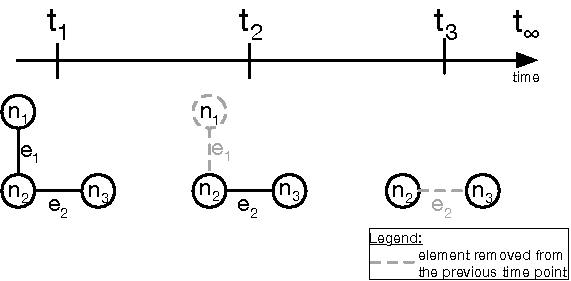
\includegraphics{img/chapt-tkm/validityExample}
	\caption{Evolution of a temporal graph over time}
	\label{fig:tkm:validityEx}
\end{figure}

In order to augment the graph with a temporal dimension, the relation $V^T$ is added.
So now the knowledge $K$ is defined as a temporal graph such as $K = (N, E, V^T)$.

A node is considered valid either until it is removed or until one of its attributes value changes. 
In the latter case, a new node with the updated value is created.
Whilst, an edge is considered valid until either its source node and target node is valid, or until the edge itself is removed.
Otherwise, nodes and edges are considered invalid.
The temporal validity relation is defined as $V^T: N \cup E \rightarrow I$.
It takes as a parameter a node or an edge ($k \in N \cup E$) and returns a time interval ($i \in I$, \cf Section~\ref{sec:tkm:timeDef}) during which the graph element is valid.

Figure~\ref{fig:tkm:validityEx} shows an example of a temporal graph $K_1$ with three nodes ($n_1$, $n_2$, and $n_3$) and two edges ($e_1$ and $e_2$) over a lifecycle from $t_1$ to $t_3$.
In this way, $K_1$ equals to $(\{n_1, n_2, n_3\}, \{e_1, e_2\}, V^{T}_1)$.
Let's assume that the graph is created at $t_1$.
As $n_1$ is modified at $t_2$, its validity period starts at $t_1$ and ends at $t_2$: $V^{T}_1(n_1) = [t_1, t_2)$.
$n_2$ and $n_3$ are not modified; their validity period thus starts at $t_1$ and ends at $t_\infty$: $V^{T}_1(n_2) = V^{T}_1(n_3) = [t_1, t_\infty)$.
Regarding the edges, the first one, $e_1$, is between $n_1$ and $n_2$ and the second one, $e_2$ from $n_2$ to $n_3$.
Both are created at $t_1$.
As $n_1$ is being modified at $t_2$, its validity period goes from $t_1$ to $t_2$:  $V^{T}_1(e_1) = [t_1, t_2)$.
$e_2$ is deleted at $t_3$.
Its validity period is thus equal to: $V^{T}_1(e_2) = [t_1, t_3)$.

\paragraph{From knowledge elements to graph nodes}
One node represent represents the state of one knowledge element during a period, the validity period.
With a temporal feature, one wants to navigate over the history of a knowledge element.
Using the temporal graph formalism, it means to access to a set of nodes.

As the validity period is defined on a right-opened interval (\cf Section~\ref{sec:tkm:timeDef}) and a new node is created as soon as the value of an existing one is modifyed, or deleted, at a time point different than the start point, then the life cycle is consistent, \ie there is no overlap between two nodes that represent the same knowledge element.

\paragraph{Lifecycle of knowledge elements}

\paragraph{Graph nodes for context}
\paragraph{Graph nodes for actions}

\paragraph{Temporal queries for requirements}
\paragraph{Temporal relations for decisions}






















\subsection{Application on the use case}

%Through this section, I will apply the formalism on the use case defined in Section~\ref{sec:intro:use-case}.
%$K_{SG}$ represents the adaptive process such as $K_{SG}=(\mathcal{C_{SG}},\mathcal{R_{SG}},\mathcal{A_{SG}}, \mathcal{D_{SG}})$.






